% 
% ======================================================================
\RequirePackage{docswitch}
% \flag is set by the user, through the makefile:
%    make note
%    make apj
% etc.
\setjournal{\flag}

\documentclass[\docopts]{\docclass}

% You could also define the document class directly
%\documentclass[]{emulateapj}

% Custom commands from LSST DESC, see texmf/styles/lsstdesc_macros.sty
\usepackage{lsstdesc_macros}
\usepackage[utf8]{inputenc}
\usepackage{graphicx}
\usepackage{subfigure}
\graphicspath{{./}{./figures/}}
\bibliographystyle{apj}

% Add your own macros here:


% 
% ======================================================================

\begin{document}

\title{ Impact of the calibration on the performances of the LSST SN survey }

\maketitlepre

\begin{abstract}
We study the impact of the LSST SN survey calibration, that is parametrized on one side as errors in the zeropoint of each filter ($\delta_{zp}$'s) and on the other as shifts in wavelength of each filter ($\delta_\lambda$'s) on the accuracy of the cosmology we will extract from LSST.
We perform a set of simulation of a typical LSST SNe Ia survey.
Then the standardization of the SNe Ia, their spectrophotometric evolution, the cosmology and the calibration parameters are fitted at the same time to capture all possible interactions between the parameters.
We show that, when all parameters are left free, a nearly complete degeneracy remains between zero points and cosmology, so that accurate external knoledge is mandatory at $1mmag$.
\end{abstract}

% Keywords are ignored in the LSST DESC Note style:
\dockeys{photometry: calibration}

\maketitlepost

% ----------------------------------------------------------------------
% 

\section{Introduction}
\label{sec:intro}

Our current knowledge of the dark energy is constrained by the SNe Ia surveys and their analysis, particulary the Joint Light-curves Analysis \cite{1401.4064} which put a constrain of 6\% on the dark energy state parameter $w$.
This uncertainty is equivalently dominated by the statistics and the systematics assiociated to these surveys and among the systematics the most important arise from the uncertainty on the calibration of the survey.
With LSST, the statistics will increase by a factor between 10 and 100. In this context the goal of this work is to study the impact of the calibration uncertainties on the performances of a LSST-like survey composed of a wide and a deep layer according to the work presented in \cite{SN-CADENCE} DESC note, by simulating a typical LSST SNe Ia dataset using \code{SnSim} and fitting a model including the standardization parameters, their spectrophotometric evolution, the cosmology and the calibration parameters at the same time to the simulated data. The performances are evaluated by the calculus of the Figure of Merit (FoM).

In section \ref{sec::simulated_dataset} we highlight the observing conditions we use in this forecast work to do the simulation of the SNe Ia and we check the quality of the light curves obtained.
We present our analysis model for the simulated dataset and the way we handle the calibration uncertainties in \ref{sec::analysis_model}.
We present our results concerning the performances of the survey for different calibration strategies in section .
In \ref{sec::discussion} we discuss the results and we conclude concerning the calibration minimal specifications in \ref{sec::conclusions}.

% ----------------------------------------------------------------------

% \section{State of the art : JLA}
% \label{sec::jla}

% Présentation des résultats JLA, description de la calibration \\
% Comparaison entre l'impact des systématiques et celui des incertitudes statistiques \\
% Ouverture sur la stat de LSST: super statistique gâchée si pas d'amélioration sur les systématiques, dont la principale est la calibration \\
% Demande une assez grosse discussion avec le groupe pour savoir ce que l'on met dans cette partie

% ----------------------------------------------------------------------

\section{Simulated dataset}
\label{sec::simulated_dataset}

\subsection{Cadence}
\label{subsec::cadence}

The LSST SN survey will be splitted in two different layers:
\begin{itemize}
\item A wide survey that will be composed of small time exposures over a large fraction of the sky.
  It would allow to discover a large number of nearby SNe Ia.
\item A deep survey inwhich a small number of fields will be observed but with high exposure times to ensure we get distant SNe Ia.
\end{itemize}
The exact cadence of the LSST SN survey is still in discussion and the results that will be presented below are likely to change.
At the moment the LSST Operations Simulator (\code{OpSim}) last results (\code{Minion\_1016}) are pessimistic: according to \cite{SN-CADENCE} the cadence of the wide and the exposure times of the deep layer are too small.
For the moment we rely on the work presented in (REF REF REF papier cadence), which proposes to use a rolling cadence for the wide survey and increase the exposure times of the deep. The nominal scenarii for the wide and the deep layer shown in \cite{SN-CADENCE} are detailed in Table \ref{tab:nominal_scenario_wide} and \ref{tab:nominal_scenario_DDF} respectively.

\begin{table*}[t]
\begin{center}
\caption{A nominal scenario for the wide that allows to build a SN
  sample complete up to $z \sim 0.4$.}
\label{tab:nominal_scenario_wide}
\begin{tabular}{l|cccc}
\hline
\hline
              & $g$ & $r$ & $i$ & $z$ \\
\hline 
$T_{exp}$      & 30       &   30    &  30        & 30       \\
$m_{5\sigma}$  &  24.83   &  24.35   &  23.88    &  23.30   \\
cadence       &  \multicolumn{4}{c}{3 days} \\
Target amplitude SNR & $>30$ & $>40$ & $>30$ & $>20$ \\
\hline
\end{tabular}
\end{center}
\end{table*}

\begin{table*}[t]
\begin{center}
\caption{A nominal scenario for the DDF that allows to build a SN
  sample complete up to $z \sim 0.75$.}
\label{tab:nominal_scenario_DDF}
\begin{tabular}{l|cccc}
\hline
\hline
              & $r$ & $i$ & $z$ & $y$ \\
\hline 
$T_{exp}$      & 1200 & 1800 & 1800 & 1800 \\
$m_{5\sigma}$  & 26.43    & 26.16    &  25.56    &  24.68   \\
cadence       &  \multicolumn{4}{c}{3 days} \\
Target amplitude SNR & $>25$ & $>60$ & $>35$ & $>20$ \\
\hline
\end{tabular}
\end{center}
\end{table*}

In our foecast we use a regular cadence based on the previous data. We suppose that every epoch will be performed and that we will suffer no lost due to bad weather for example.

\subsection{Instrument Model and Observing conditions}

Concerning the instrument model and still relying on \cite{SN-CADENCE} we use the most recent model from \cite{SMTN-002} (SMTN-002). The previous model, described in \cite{LSE-40} (LSE-40) has been revised and the new troughput is 40\% lower  in SMTN-002.
Concerning the observing conditions, we use median conditions (same for all epoch), we can see these values for each filter in the Figure \ref{fig:zp} extracted from \cite{SN-CADENCE}.

\begin{figure}[t]
\begin{center}
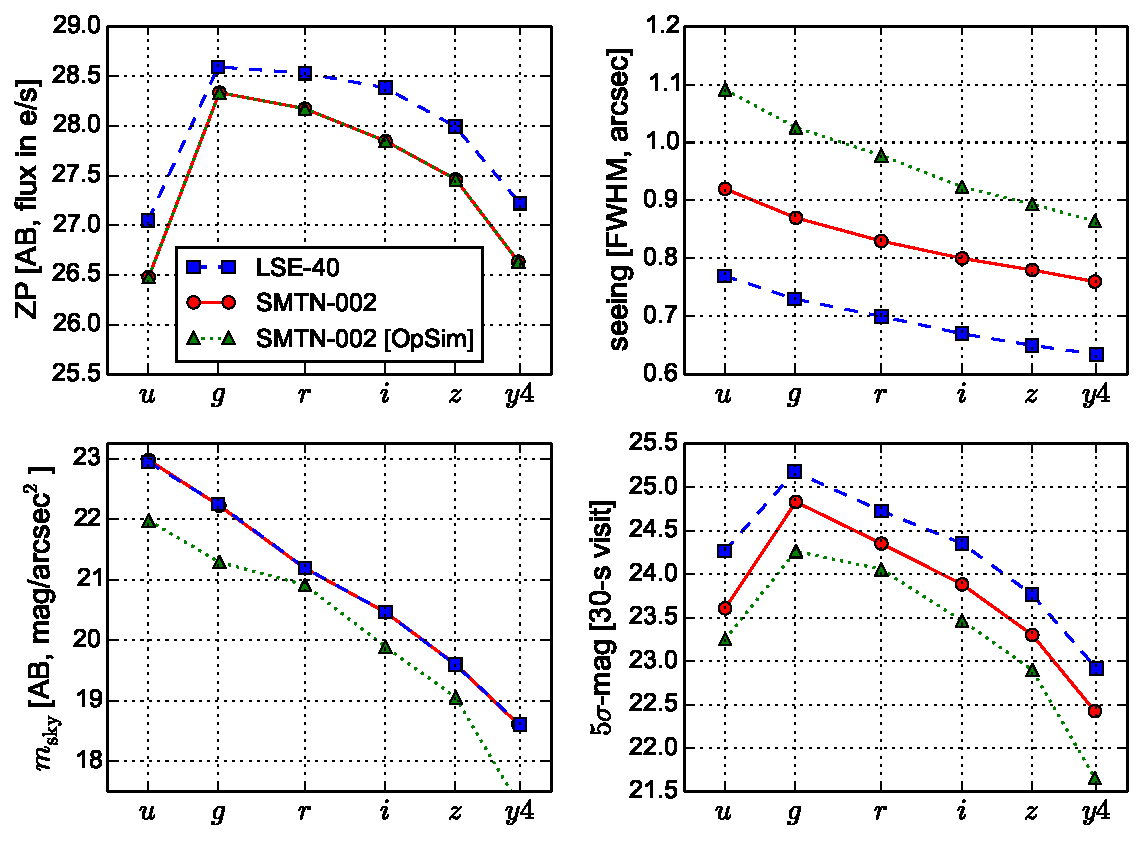
\includegraphics[width=\linewidth]{lsst_model_summary.pdf}
\caption{Parameters of the survey simulation : from left to right and top to bottom we have : zero-points, median seeing, dark sky mags and limiting mags, from \cite{SN-CADENCE} in each $grizy$ band.}
\label{fig:zp}
\end{center}
\end{figure}

\subsection{Simulated SNe}
\label{ssec::snsim}
We use \code{SnSim} to produce the observed SNe Ia and their light curves with the cadence and observing conditions detailed in the previous parts.
Our study is performed for 1 year of wide and 4 years of deep layers.
The repartition in reshift of the simulated SNe Ia is shown in Figure \ref{fig:z_distrib}. We used 4 years of deep and 1 year of wide to get the same number of SNe.
\begin{figure}[ht]
  \centering
  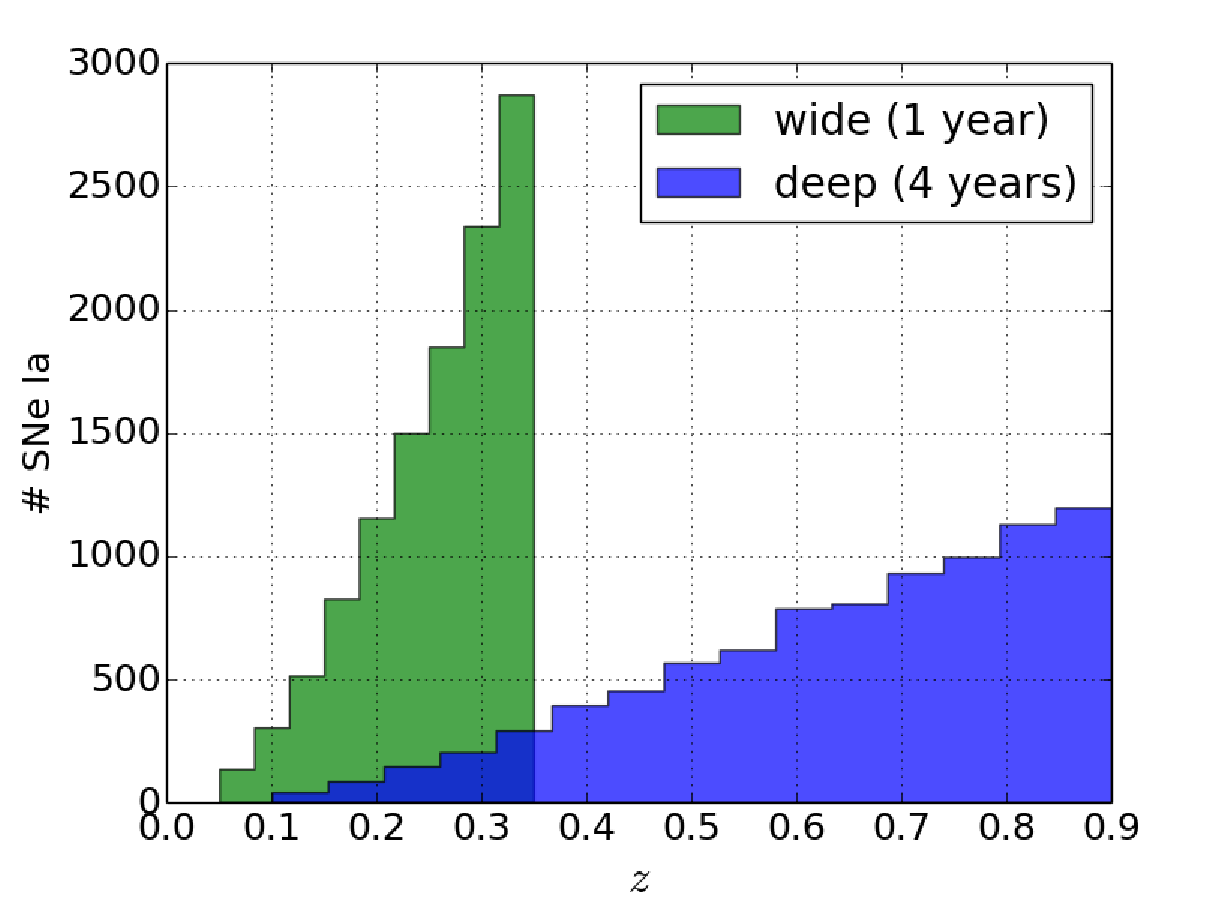
\includegraphics[width=\linewidth]{z_surveys_population.pdf}
  \caption{Redshift distribution of the SNe Ia simulated with 4 years of deep layer and 1 year of wide for a total of $\approx 20\times10^3$ SNe Ia.}
  \label{fig:z_distrib}
\end{figure}
In Figure \ref{fig:lc_examples} we show that in two extrem cases of SNe Ia, one from the wide layer at $z=0.06$ and one from the deep layer at $z=0.87$, the light curves we obtained are well sampled in time and the uncertainty associated to each flux measurement is reasonably low compared to the light curve amplitude..

\begin{figure*}[t]
\begin{center}
\subfigure[$z = 0.06$]{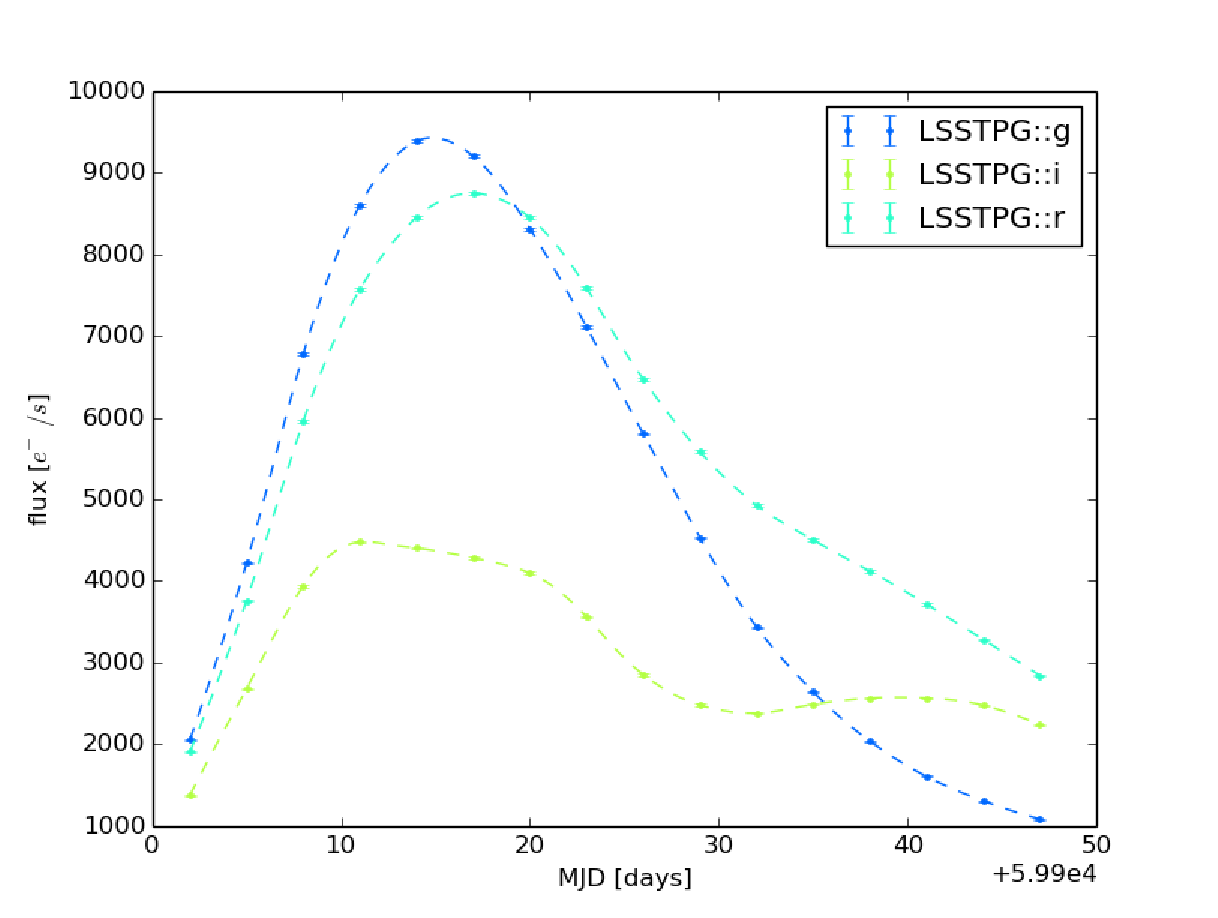
\includegraphics[width=0.48\linewidth]{lc_sn_z006.pdf}}
\subfigure[$z = 0.87$]{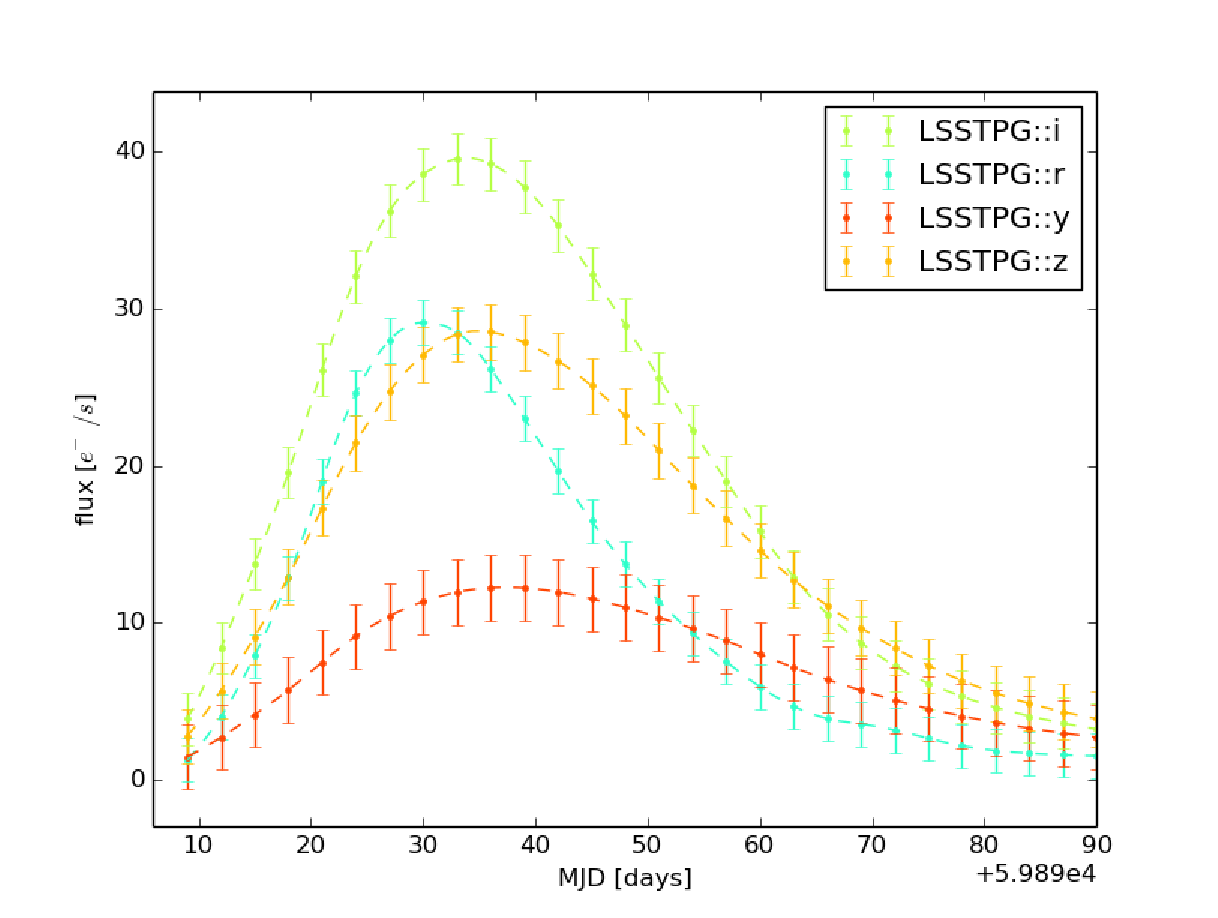
\includegraphics[width=0.48\linewidth]{lc_sn_z087.pdf}}\\
\caption{Light curves for a SN Ia measured in the wide layer at $z=0.06$ in $gri$ bands (left) and a SN Ia measured in the deep layer at $z=0.87$ in $rizy$ bands (right).}
\label{fig:lc_examples}
\end{center}
\end{figure*}

Finally, we show in Figure \ref{fig:sigmas} that in each layer the color $c$, the time of maximum luminosity $t_0$ and the stretch of the simulated SNe Ia are well constrained over their redshift range.

\begin{figure*}[t]
\begin{center}
\subfigure[wide]{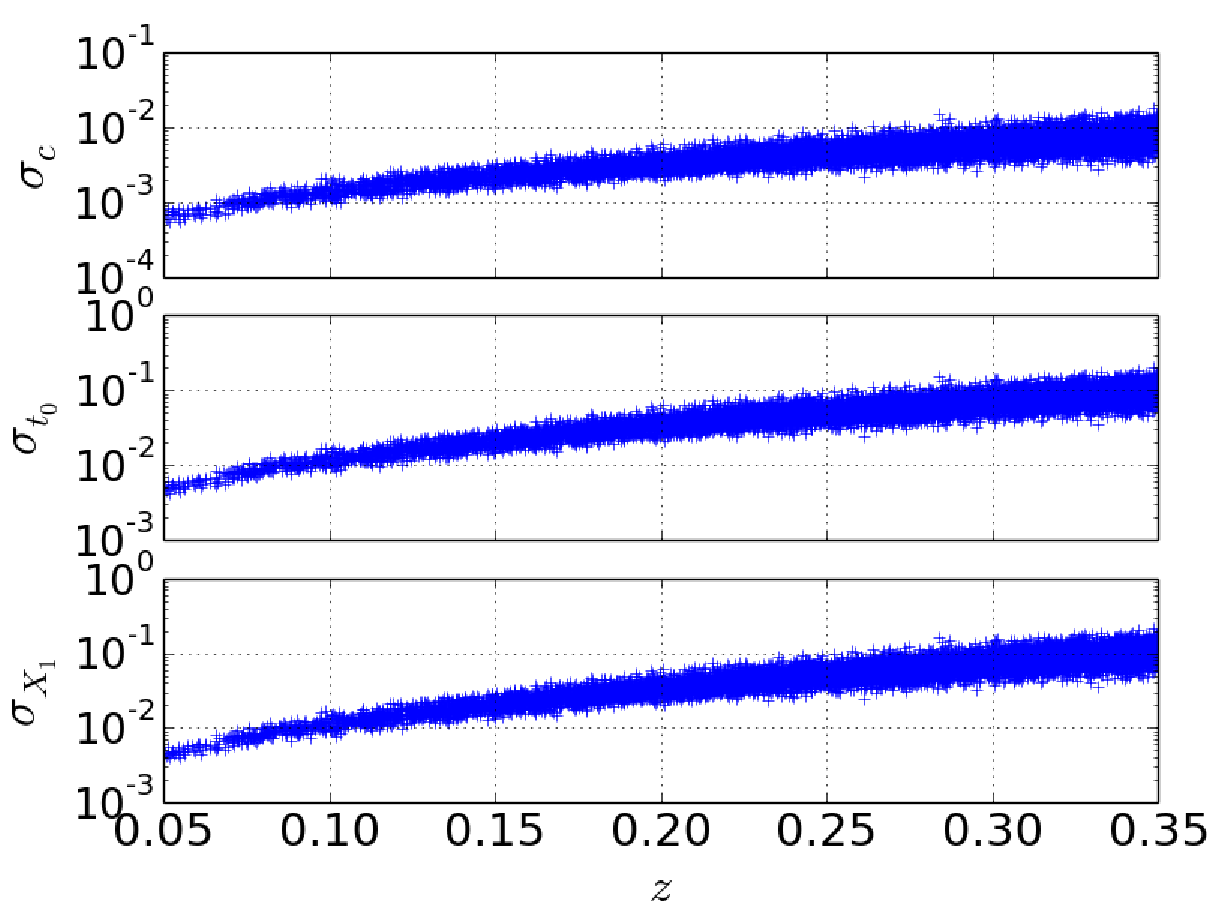
\includegraphics[width=0.48\linewidth]{sigmas_wide.pdf}}
\subfigure[deep]{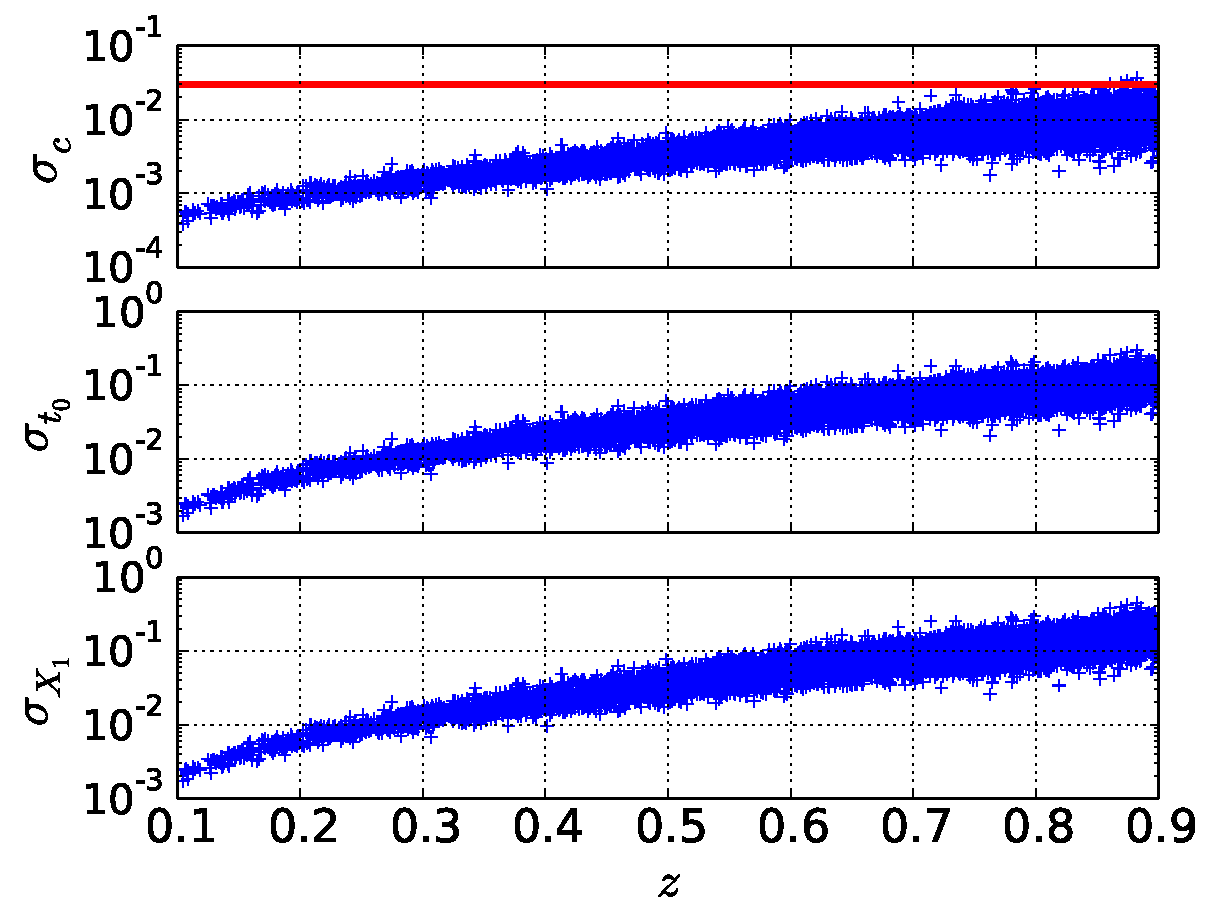
\includegraphics[width=0.48\linewidth]{sigmas_deep.pdf}}\\
\caption{Uncertainty of the color, the time of maximum luminosity and the stretch of each SN Ia (from top to bottom) in the wide (left) and the deep (right) layers.}
\label{fig:sigmas}
\end{center}
\end{figure*}

% ----------------------------------------------------------------------

\section{Analysis Model}
\label{sec::analysis_model}

\subsection{Model details}
\label{subsec::model_details}
Our model has to be representative of the errors, meaning it has the same number of degrees of freedom as the typical model that will be use for the analysis of the LSST SNe Ia survey data.
This also have to be a light-weighted simulation to allow us to iterate over a large set of different entry parameters.
Then our simulated sample contains only photometric data and no SN Ia spectra.
The calibration uncertainties induce redshift dependent errors on magnitude and color.
It is thus of primary importance to account for all the spectral effects in order to accurately propagate calibration uncertainties.
On the contrary light-curve shapes (stretch) is expected to be well constrained thanks to the good sampling (\ref{ssec::snsim}), and calibration uncertainties do not strongly impact shapes (e.g. \cite{1401.4064} Figure 6).
We then choose to skip the time dependant part to simplify the simulation, by only using the flux of each measured SN Ia in each used band, interpolated at the day of maximum luminosity in the restframe $B$ band (hereafter DayMax).
Then the flux of a given SN Ia measured at DayMax in a band $b$ can be modelized as follows:

\begin{equation}
  \varphi_b = \frac{1}{1+z} \times \frac{10^{-10}}{d_L^2(z, \theta_\text{c})}\times \int \lambda S(\frac{\lambda}{1+z}) T_b(\lambda) d\lambda \text{ ,}
\end{equation}
where $z$ and $d_L$ are respectively the redshift and the luminosity distance of the given supernova,
$\theta_\text{c}$ is the vector of the cosmological parameters (depending on the model we choose to use),
$S(\frac{\lambda}{1+z})$ is the SED of a standard SN Ia that describes its restframe spectrophotometric evolution with wavelength
and $T_b(\lambda)$ is the transmission of the detector in a band $b$.
To describe simultaneously the flux emitted by all our generated sample of SNe in each band at DayMax we choose to work in magnitudes ($m=-2.5 log\varphi$) for the model to be more linear.
The observer frame magnitude of a supernova at a redshift $z$ in a band $b$ as follows:
\begin{equation}
\begin{split}
\label{eq::raw_model}
m_b = &\mu(z, \theta_\text{c}) + 25 + 2.5log_{10}(1+z) \\
&- 2.5log\int \lambda S(\lambda) T_b(\lambda) d\lambda \text{ ,}
\end{split}
\end{equation}
where $\mu(z, \theta_\text{c})$ is its distance modulus related to the luminosity distance $d_L$ as $\mu(z, \theta_\text{c}) = 5log_{10}(d_L)$.
Then we perform a Taylor expansion around the mean position of the passband:

\begin{equation}
\begin{split}
\int \lambda S(\lambda) T_b(\lambda) d\lambda = \int \lambda \left( S(\bar\lambda_b ) +(\lambda - \bar\lambda_b )\frac{\partial S(\bar\lambda_b )}{\partial \lambda} \right) T_b(\lambda) d\lambda
%S(\bar\lambda_b ) \int \lambda T_b(\lambda) d\lambda + \frac{\partial S(\bar\lambda_b )}{\partial\lambda} \int \lambda (\lambda - \bar\lambda_b ) T_b(\lambda) d\lambda
\end{split}
\end{equation}
If we choose $\bar\lambda_b $ to be:
\begin{equation}
  \bar\lambda_b  = \frac{\int \lambda^2 T_b(\lambda) d\lambda}{\int \lambda T_b(\lambda) d\lambda}
\end{equation}
The first order terms are set to zero, so we have:
\begin{equation}
\int \lambda S(\frac{\lambda}{1+z}) T_b(\lambda) d\lambda = S(\frac{\bar\lambda_b }{1+z}) \times \int \lambda T_b(\lambda) d\lambda
\end{equation}
Thus our model in eq \ref{eq::raw_model} becomes:          
\begin{equation}
  m_b = \mu(z, \theta_\text{c}) + 25 + 2.5log_{10}(1+z) - 2.5 log_{10} S(\bar\lambda_b ) + \mathcal{Z}_b \text{ ,}
\end{equation}
where $\mathcal{Z}_b = -2.5 log \int \lambda T_b(\lambda) d\lambda$ is the band zeropoint.

As we will show later, care must be taken while modelizing the spectrophotometric evolution of the supernovae and its characterization shall remain free to evolve with the input data.
We decompose $-2.5log_{10}S(\bar\lambda_b)$ on 3 different terms:
\begin{equation}
-2.5log_{10}S(\bar\lambda_b) = M_X + P(\frac{\bar\lambda_b}{1+z}) + cQ(\frac{\bar\lambda_b}{1+z}) \text{ ,}
\end{equation}
where $P(\frac{\bar\lambda_b}{1+z})$ plays the role of the mean restframe spectrum of a "standard" SN Ia, through a decomposition over a third order Spline basis, $M_X$ is a normalization factor accounting for the restframe absolute luminosity of each SN and $Q(\frac{\bar\lambda_b}{1+z})$ is a color law accounting for the color variation of each SN with a polynomial of fourth degree.
We also introduce here the color $c$ of each SN.
Degeneracies rise between these different parameters, we will show how to handle them in \ref{ssec:model_deg}.
Incorporated to the model it gives:

\begin{equation}
\begin{split}
m_b = &M_X + 25 + \mu(z, \theta_\text{c}) + 2.5log_{10}(1+z) \\
&+ P(\frac{\bar\lambda_b }{1+z}) + cQ(\frac{\bar\lambda_b }{1+z})+ \mathcal{Z}_b \text{ .}
\end{split}
\end{equation}

Once the spectrophotometric model has been correctly parametrized, we have to add the standardisation parameters that will ensure the smallest dispersion of our dataset.
Since we do not work in the phase space of the light curves the only standardization parameter we use is the brighter-bluer parameter $\beta$.
It incorporates to our model as follows:
\begin{equation}
\begin{split}
\label{eq::model}
m_b = &M_X + 25 + \mu(z, \theta_\text{c}) + 2.5log_{10}(1+z) \\
&+ P(\frac{\bar\lambda_b }{1+z}) + cQ(\frac{\bar\lambda_b }{1+z}) + \textcolor{red}{c\beta}+ \mathcal{Z}_b
\end{split}
\end{equation}

% ----------------------------------------------------------------------

\subsection{Calibration parameters}
\label{sec::calib_uncertainties}
The core of this work is about the way we handle the calibration errors and incorporate them in \ref{eq::model}.
We choose to parametrize them in two different subsets of parameters:
\begin{itemize}
\item $\delta zp$'s, that takes into account the error we make on the normalization of the transmission in each band.
There is one associated to each filter we use.
\item $\delta \lambda$'s, which is the error made in observer frame on the wavelength position of each filter. 
\end{itemize}

Our model then becomes :
\begin{equation}
\begin{split}
m_b = & M_X + 25 + \mu(z, \theta_\text{c}) + 2.5log_{10}(1+z) + \mathcal{Z}_b \\
&+ P(\frac{\bar\lambda_b  + \textcolor{red}{\delta\lambda_b}}{1+z}) + cQ(\frac{\bar\lambda_b  + \textcolor{red}{\delta\lambda_b}}{1+z}) + {c\beta} + \textcolor{red}{\delta zp_b}
\end{split}
\end{equation}
These calibration parameters are associated to a calibration covariance matrix $C_s$.
Non-diagonnal terms in $C_s$ should rise depending on the calibration strategy.
The state of the art concerning SNe Ia flux measurements consists in comparing their flux directly with calibrated astrophysical standards.
We suppose that the zeropoint of a band $b$ is obtained using the flux measurement of this calibrated astrophysical standard, which is modelized as:
\begin{equation}
zp_b = \int T_b(\lambda) S_{std}(\lambda) d\lambda + n_b
\end{equation}
Where $T$ is the transmission of the instrument, $S_{std}$ is the spectrum of the astrophysical standard and $n_b$ is a random noise whith $cov(n_b) = \sigma_{zp_b}^2$.
This way of measuring flux leads to the fact that if we make an error on the wavelength position of the filters, the flux integration of the standard will not be what we should expect and thus leads to an error on the zeropoint of the band.
In fact we have:
\begin{equation}
\begin{split}
zp_b &= \int \bar T_b(\lambda) S_{std}(\lambda) d\lambda + n_b + \frac{\partial \int{T_b(\lambda)S(\lambda)d\lambda}}{\partial \bar\lambda_b }\\
&= \bar{zp}_b + e_{zp_b} + \frac{\partial zp_b}{\partial \bar\lambda_b }\delta\bar\lambda_b 
\end{split}
\end{equation}
We then have:
\begin{equation}
\begin{pmatrix}
  zp \\
  \bar\lambda_b 
\end{pmatrix}
=
\begin{pmatrix}
  1 & \frac{\partial zp}{\partial \lambda} \\
  0 & 1
\end{pmatrix}
\begin{pmatrix}
  e_{zp} \\
  \delta\bar\lambda_b 
\end{pmatrix}
+
\begin{pmatrix}
  \bar{zp} \\
  0
\end{pmatrix}
\end{equation}
From this phenomenon raise correlation terms between $\delta \lambda$ and $\delta zp$ for a same band.
We define $\frac{\partial zp}{\partial \lambda}$ as the change in zeropoint for $1 \AA$ of filter position error, obtained by comparing the integrated flux of an astrophysical standard (P330E in this case) in a reference filter and in a shifted filter.
We have:
\begin{equation}
C_s = cov
\begin{pmatrix}
  zp \\
  \bar\lambda_b 
\end{pmatrix}
=
\begin{pmatrix}
  1 & \frac{\partial zp}{\partial \lambda} \\
  0 & 1
\end{pmatrix}
C_{s1}
\begin{pmatrix}
  1 & 0 \\
  \frac{\partial zp}{\partial \lambda} & 1
\end{pmatrix}
\end{equation}
We put the values in Table \ref{tab::calib_derivatives}, then $C_s$ becomes :
\begin{equation}
\label{eq::cov_calib}
C_s = 
\begin{pmatrix}
  \sigma^2_{ zp_{g}} + (\sigma_{\lambda_g} \frac{\partial zp_g}{d\lambda_g})^2 & 0 & \frac{\partial zp_g}{\partial \lambda_g} \sigma^2_{ \lambda_g} & 0 \\
   0 & \ddots & 0 & \ddots \\
   \frac{\partial zp_g}{\partial \lambda_g} \sigma^2_{ \lambda_g} & 0 & \sigma^2_{\lambda_{g}} & 0 \\
   0 & \ddots & 0 & \ddots 
\end{pmatrix}
\end{equation}

\begin{table*}[t]
\begin{center}
\caption{$\delta zp$'s derivatives with $\delta\lambda$'s computed using P330E spectrum.}
\label{tab::calib_derivatives}
\begin{tabular}{l|ccccc}
\hline
\hline
  & $g$ & $r$ & $i$ & $z$ & $y$ \\
\hline 
  $\frac{\partial\delta zp}{\partial\delta \lambda}$ $(mmag/\AA)$& 0.026 & 0.18 & 0.24 & 0.23 & 0.22\\
\hline
\end{tabular}
\end{center}
\end{table*}

% ----------------------------------------------------------------------

\subsection{Model degeneracies}
\label{ssec::model_deg}

At this current stage our model have some degeneracies that we must get rid of.
The way to handle this degeneracies is to add priors to our model.
If $J$ is the matrix of the derivatives  of our model with respect to all free parameters (columns) for all light curve amplitudes measured (lines), we can vertically add matrices to $J$ for each prior, corresponding to one or more "additionnal" measurements:
\begin{equation}
J =
\begin{pmatrix}
  J \\
  J_\text{priors}
\end{pmatrix} 
\end{equation}

In parallel, if $C$ is the covariance matrix of our measurements, we add diagonally the covariance matrix of the prior to $C$:
\begin{equation}
C =
\begin{pmatrix}
  C & 0 \\
  0 & C_\text{priors}
\end{pmatrix} 
\end{equation}

In our case we add the following priors:
\begin{itemize}
\item The spectrum normalization, to cut degeneracy with the distance modulus $\mu$ that could increase while $M_X$ decrease.
\item The spectrum color, that is degenerated with the color law.
\item The fact that the color law is fixed at $\lambda_B$ and $\lambda_V$ respectively mean wavelength of the $B$ and $V$-bands
\item We fix the dispersion of the $M_X$'s at 14\% because otherwise we have degeneracies with the distance moduli.
\item Since we use a $w_0w_a$ cosmology, $\theta_\text{c} = \{ \Omega_m$, $\Omega_k$, $w_0$, $w_a$, $H_0$, $\Omega_bh^2 \}$, we add a Planck prior, extracted from Planck 2015 results(\cite{1502.01589}), which brings us the information on $H_0$ and $\Omega_k$ we wouldn't get with the SNe Ia only.
\end{itemize}


% ----------------------------------------------------------------------

\subsection{Error propagation}
\label{sec::linalg}

If we linearize our model $\mathcal{M}$, we have:
\begin{equation}
\mathcal{M} = J \times \vec\theta
\end{equation}
Where $J$ is called the "jacobian" matrix and contains the derivatives of our model with respect to all free parameters (columns) for all light curve amplutude measured (lines) and $\vec\theta$ the vector of all our free parameters (details in Table \ref{tab:params}).

\begin{table*}[t]
\begin{center}
\label{tab:params}
\caption{Summary of our model free parameters}
\begin{tabular}{l|ccccccccc}
\hline
\hline
Free parameters & $M_X$ & $\theta_\text{c}$ & $\theta_P$ & $\theta_Q$ & $c$ & $\beta$ & $\mathcal{Z}$ & $\delta zp$ & $\delta \lambda$ \\
\hline
\# parameters & $N$ & 6 & 31 & 5 & $N$ & 1 & 5 & 5 & 5 \\
\hline
\end{tabular}
\end{center}
\end{table*}


We will perform a simultaneous fit marginalized over all Table \ref{tab:params} parameters, but has we can see there's a lot of them, so to ensure a quicker execution and avoid memory issues we work with sparse matrices.

The fit is performed by minimizing the following $\chi^2$:
\begin{equation}
\chi^2 = \sum_{sb}\frac{[m_{sb} - \mathcal{M}(s, b, \vec\theta)]^2}{\sigma_{sb}}
\end{equation}
The normal equation for this $\chi^2$ is:
\begin{equation}
J^TC^{-1}J = J^TC^{-1}y
\end{equation}
where $C$ is the covariance matrix of the measurements.

Finally we add the calibration covariance matrix $C_s$ (explicited in \ref{sec::calib_uncertainties}) as a prior to our model (as in \ref{sec::model_deg}).
For the moment we have to keep in mind that these value are not fixed, and we are going to make this study for several examples of what would be the calibration accuracy for the LSST SN survey.

Since we want to study the performances of the survey, we do not need to perform a fit.
The relevant quantity is the Fisher matrix, that we call $H$
\begin{equation}
H = J^TWJ
\end{equation}
where $W = C^{-1}$.
The inverse of $H$ is the covariance matrix of all the free parameters.

% ----------------------------------------------------------------------

\section{Results}
\label{sec::results}
We study the performances through the FoM, we have:
\begin{equation}
FoM = \frac{1}{\sqrt{det(cov(w_0, w_a))}}
\end{equation}
We can then only perform a block inversion of $H$.
We modify the calibration strategy by changing the $\sigma_{\delta \lambda}$'s and the $\sigma_{\delta zp}$'s in $C_s$ (eq \ref{eq::cov_calib}) which is included in $H$ through $W$.
In a first time we vary a same value for all the $\sigma_{\delta zp}$'s while we fix the $\delta \lambda$'s.
We compute the $FoM$ for each common value of the $\sigma_{\delta zp}$'s, we present this result in Figure \ref{fig:fom_zp}.
On this figure we an see that a transition in the level of performances occurs around $\sigma_{\delta zp} = 10^{-3}$.
If we consider that the current uncertainties on the $\delta zp$'s is around $5 \times 10^{-3}$ (\cite{1401.4064}), we note that we need improvements to extract the most information from the statistics granted by one year of the survey.
When doing the same analysis with the filter position parameters we notice that there is no evolution of the performances when improving the accuracy of the $\delta\lambda$'s. This is explained by the fact that the filters positions are calibrated by the SNe Ia, as we can see in figure \ref{fig:delta_lambda_ev} above an a priori uncertainty on the filter position of $\approx 1A$, the a posteriori uncertainty obtained with $H$ saturates at $1 \AA$. We come back to this in the discussion.

\begin{figure}[ht]
  \centering
  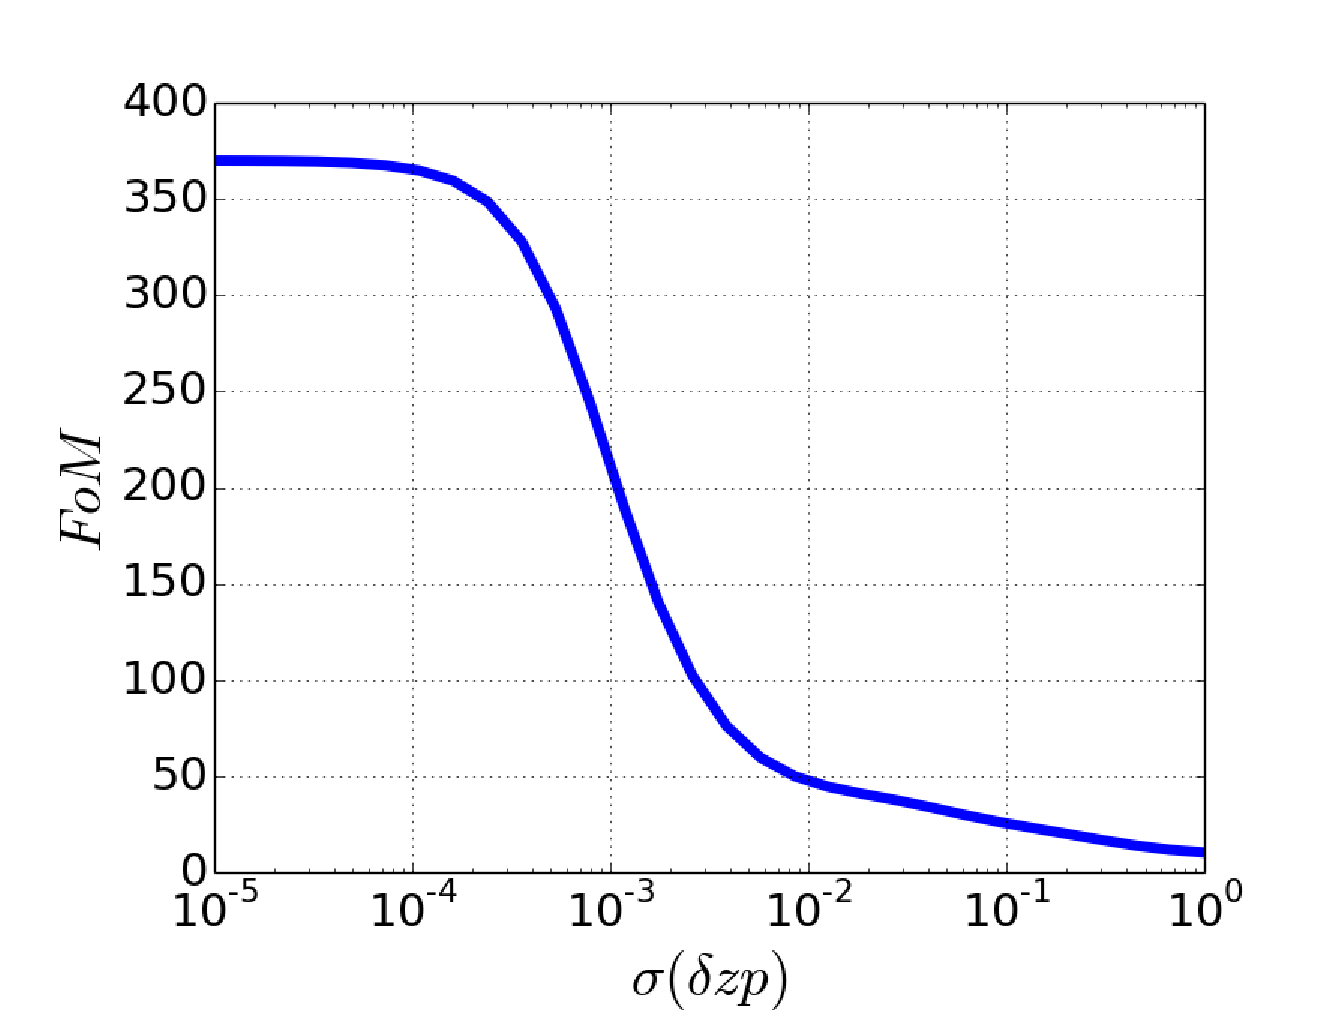
\includegraphics[width=\linewidth]{FoM_20k.pdf}
  \caption{Evolution of the $FoM$ with the uncertainty on the $\delta zp$'s.}
  \label{fig:fom_zp}
\end{figure}

\begin{figure}[ht]
  \centering
  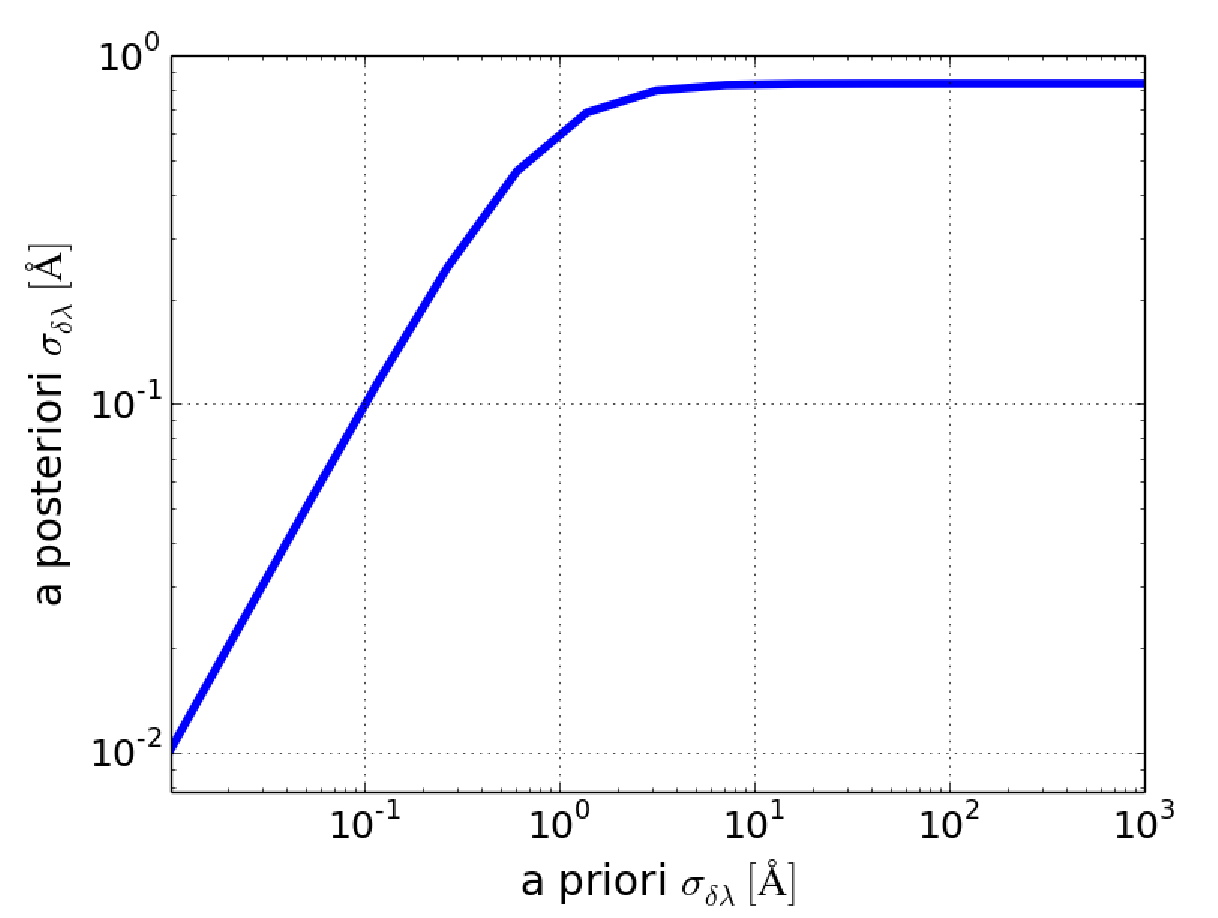
\includegraphics[width=\linewidth]{a_posteriori_sigmas.pdf}
  \caption{Evolution of the uncertainty on the filter position extracted from the free parameters covariance matrix $H$ with the uncertainty ont the filter position as entry parameters in the measurements covariance matrix $C_s$.}
  \label{fig:delta_lambda_ev}
\end{figure}

As a parallel work, we wanted to study what would be this results without the training of our spectrophotometric model, that is by not considering $\theta_P$ as free parameters.
The figure \ref{fig:fom_wout_training} shows that, compared to what we obtain with the training, we are making a large overestimation of the performances of the survey, and we would think that the calibration does not need to be that precise. That is why we have to take care with handling the spectrophotometric model.
\begin{figure}[ht]
  \centering
  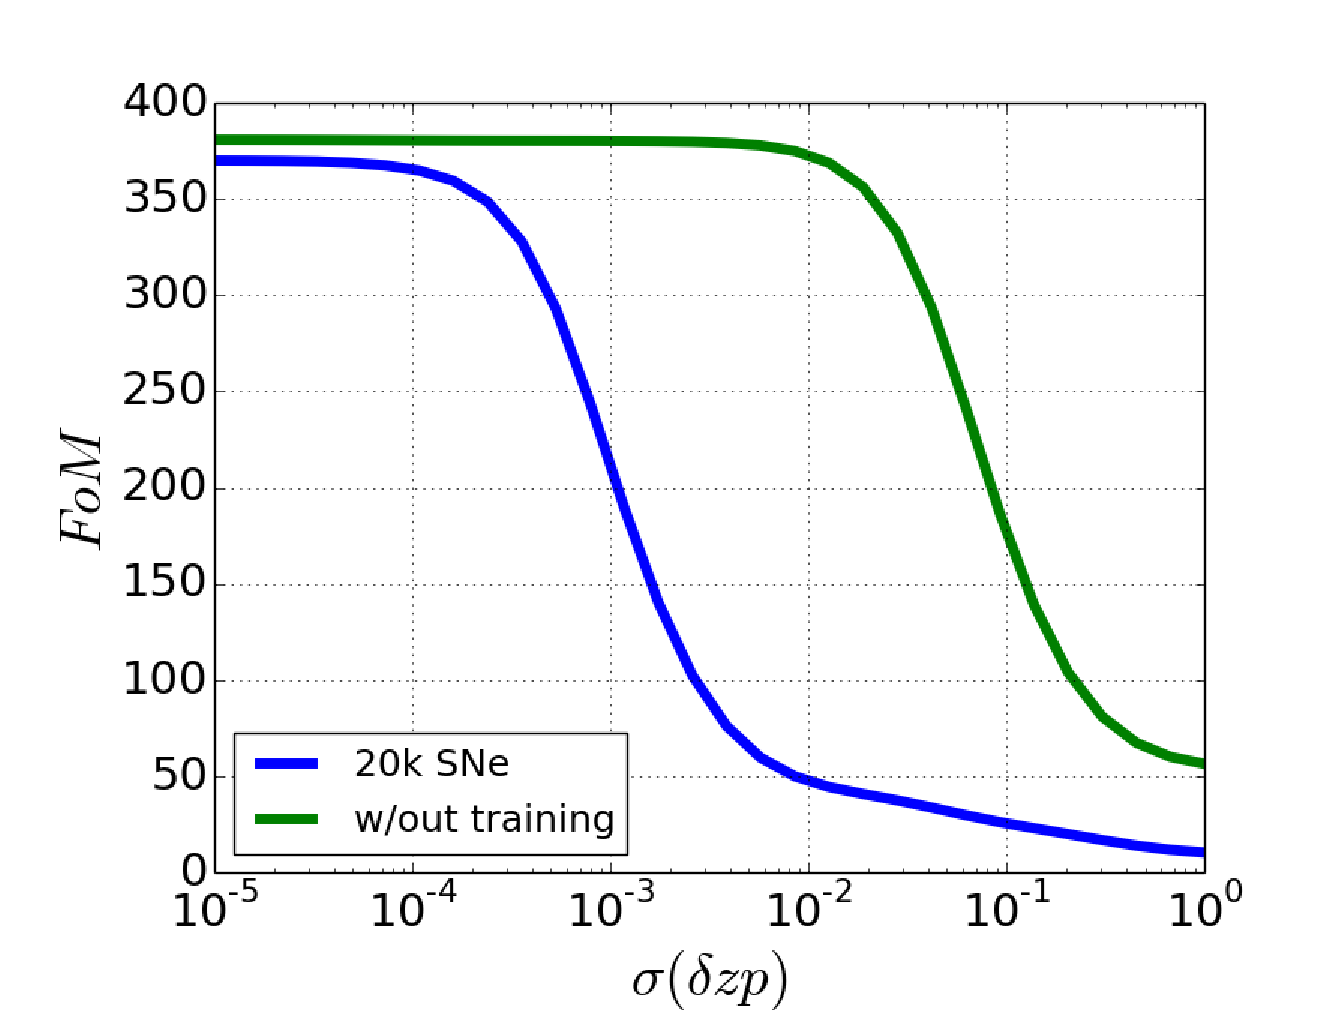
\includegraphics[width=\linewidth]{FoM_20k+training.pdf}
  \caption{Evolution of the $FoM$ with the uncertainty on the $\delta zp$'s with and without the spectrophotometric model training}
  \label{fig:fom_wout_training}
\end{figure}

% ----------------------------------------------------------------------

\section{Discussion}
\label{sec::discussion}
First we can notice that in Fig \ref{fig:fom_zp} the $FoM$ is different from 0 even when the knowledge on the zero-points is minimal.
This auto-calibration of the zero-points is an artifact assuming a perfectly calibrated SN model.
Concerning the auto calibration of the filter positions, we can notice that, assuming a smooth cosmology, there does not seem to be degeneracies between the filter positions and cosmological parameters.
This is because Filter shifts introduce wiggles in the Hubble Diagram that can be spotted and erased by the fit.
Caution should be exercised on three points:
\begin{itemize}
\item we assume a perfectly known redshift.
\item there is no high frequency spectral features in our photometric SN model
\item this suppose spatial homogeneity of the filters so that the error in filters positions is common to all SNe and reflects as unexpected coherent features on the Hubble Diagram rather than as an invisible extra noise.
\end{itemize}

% ----------------------------------------------------------------------

\section{Conclusions}
\label{sec::conclusions}

We show in this study that we can expose a relation between the calibration  parameters uncertainties and the performances of a LSST SN survey by using a model fitting simultaneously the spectrophotometric evolution of the SNe Ia, the cosmology and the calibration parameters.
We have also shown the necessity to take into account the trainging of the spectrophotmetric model over the dataset to obtain realistic results from this type of study.
The exposed relation highlights the necessity to calibrate the troughput of our filters below the $10^{-3}$ level in order to exploit at a good level the increase of statistics that LSST will bring.
Finaly we found that the uncertainty on the filters positions shows to have no effect on the performances since it is calibrated by the well constrained dataset. This particular point will be investigated in a second iteration of this work, in a first time by adding an uncertainty on the redshift of each SN and in a second time by adding the phase dimension of the spectrophotometric evolution of the SNe Ia.


% ----------------------------------------------------------------------

\subsection*{Acknowledgments}

%Here is where you should add your specific acknowledgments, remembering that some standard thanks will be added via the \code{acknowledgments.tex} and \code{contributions.tex} files.

% 
This is the text imported from \code{acknowledgments.tex}, and will be replaced by some standard LSST DESC boilerplate at some point.
% 


\input{contributions}

%{\it Facilities:} \facility{LSST}

% Include both collaboration papers and external citations:
\bibliography{lsstdesc,main}

\end{document}
% ======================================================================
% 
